\section{Spenntrær}
Vi begynner med en definisjon:\index{spenntre} \index{minimalt spenntre}

\begin{definition}
Et \textbf{spenntre} for en urettet graf $ G $ er et tre med kanter fra grafen slik at alle nodene i $ G $ er forbundet. Spesielt er et \textbf{minimalt spenntre} de(t) spenntre(ene) med lavest total kostnad.
\end{definition}

\noindent Minimale spenntrær er sjeldent entydig bestemt. Vi har et entydig minimalt spenntre hvis alle kantene har forskjellig vekt. Vi tegner opp et eksempel:

\begin{figure}[h!]
\centering
\caption{En graf (venstre) og et minimalt spenntre for grafen (høyre)}~\\
\label{fig:min_spenntre}
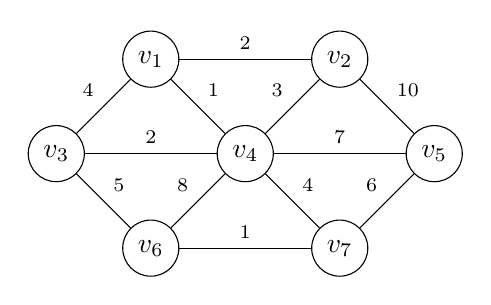
\begin{tikzpicture}[auto,node distance=2cm, scale=0.8]
\tikzstyle{vertex} = [circle, draw=black]
\tikzstyle{edge} = [draw=black]

\node[vertex] (v1) at (-1.5,1.5) {$ v_1 $};
\node[vertex] (v2) at (1.5, 1.5) {$ v_2 $};
\node[vertex] (v3) at (-3,0) {$ v_3 $};
\node[vertex] (v4) at (0,0) {$ v_4 $};
\node[vertex] (v5) at (3,0) {$ v_5 $};
\node[vertex] (v6) at (-1.5,-1.5) {$ v_6 $};
\node[vertex] (v7) at (1.5,-1.5) {$ v_7 $};

\draw[edge] (v3) to node{\scriptsize4} (v1);
\draw[edge] (v3) to node{\scriptsize2} (v4);
\draw[edge] (v3) to node{\scriptsize5} (v6);
\draw[edge] (v1) to node{\scriptsize1} (v4);
\draw[edge] (v6) to node{\scriptsize8} (v4);
\draw[edge] (v4) to node{\scriptsize3} (v2);
\draw[edge] (v4) to node{\scriptsize4} (v7);
\draw[edge] (v4) to node{\scriptsize7} (v5);
\draw[edge] (v2) to node{\scriptsize10} (v5);
\draw[edge] (v7) to node{\scriptsize6} (v5);
\draw[edge] (v1) to node{\scriptsize2} (v2);
\draw[edge] (v6) to node{\scriptsize1} (v7);
\end{tikzpicture}~~
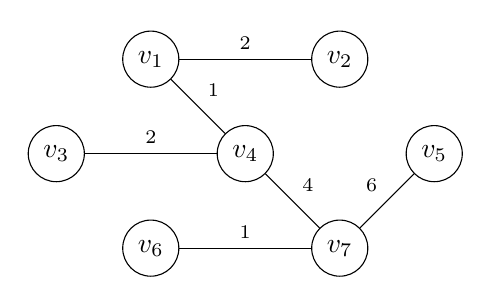
\begin{tikzpicture}[auto,node distance=2cm, scale=0.8]
\tikzstyle{vertex} = [circle, draw=black]
\tikzstyle{edge} = [draw=black]

\node[vertex] (v1) at (-1.5,1.5) {$ v_1 $};
\node[vertex] (v2) at (1.5, 1.5) {$ v_2 $};
\node[vertex] (v3) at (-3,0) {$ v_3 $};
\node[vertex] (v4) at (0,0) {$ v_4 $};
\node[vertex] (v5) at (3,0) {$ v_5 $};
\node[vertex] (v6) at (-1.5,-1.5) {$ v_6 $};
\node[vertex] (v7) at (1.5,-1.5) {$ v_7 $};

\draw[edge] (v3) to node{\scriptsize2} (v4);
\draw[edge] (v1) to node{\scriptsize1} (v4);
\draw[edge] (v4) to node{\scriptsize4} (v7);
\draw[edge] (v7) to node{\scriptsize6} (v5);
\draw[edge] (v1) to node{\scriptsize2} (v2);
\draw[edge] (v6) to node{\scriptsize1} (v7);
\end{tikzpicture}~\\~\\
\end{figure}

For å finne et minimalt spenntre til en graf kan vi bruke Prims algoritme eller Kruskals algoritme  (se \ref{kruskal})
